\section{Метод конечных разностей во временной области}

Метод конечных разностей во временной области относится к общему классу сеточных методов решения дифференциальных уравнений. В его рамках уравнения Максвелла подвергаются дискретизации с использованием центрально-разностной аппроксимации как по временной, так и по пространственным координатам. Полученные конечно-разностные уравнения решаются программными или аппаратными средствами в каждой точке временной сетки, причём компоненты вектора напряжённости магнитного поля смещены на половину шага дискретизации относительно компонент вектора напряженности электрического поля вдоль каждой оси. Расчёт полей в ячейках сетки повторяется до тех пор, пока не будет получено решение поставленной задачи в интересующем промежутке времени.

% Базовый алгоритм FDTD; сосредоточенный резистивный источник напряжения; PML

Существует также большое количество расширений метода, наиболее популярными из которых являются разнообразные поглощающие и отражающие граничные условия, 
преобразование ближнего поля в дальнее, моделирование сосредоточенных активных и пассивных элементов. В рамках данной работы были реализованы только базовый алгоритм метода, сосредоточенные источник тока и резистивный источник напряжения, а также поглощающие граничные условия PML.

\subsection{Краткое описание метода}

Рассмотрим систему из четырёх векторных уравнений Максвелла, записанных в системе единиц СИ:
\begin{equation}
    \label{eq:MaxwellEquations}
	\begin{cases}
		\Rot\vec{E} = \sigma^{*}\vec{H}-\parder{\vec{B}}{t}, \\
		\Rot\vec{H} = \sigma\vec{E}+\parder{\vec{D}}{t}, \\
		\Div\vec{D} = \rho, \\
		\Div\vec{B} = 0.
	\end{cases}
\end{equation}

В системе~\eqref{eq:MaxwellEquations} использованы следующие обозначения:
\begin{itemize}[label={}]
\item $ \vec{E} $ --- напряжённость электрического поля,
\item $ \vec{H} $ --- напряжённость магнитного поля,
\item $ \vec{B} $ --- магнитная индукция ($ \vec{B} = \mu\mu_{0}\vec{H} $),
\item $ \vec{D} $ --- электрическая индукция ($ \vec{D} = \varepsilon\varepsilon_{0}\vec{E} $),
\item $ \varepsilon $ --- относительная диэлектрическая проницаемость,
\item $ \mu $ --- относительная магнитная проницаемость,
\item $ \sigma $ --- удельная электрическая проводимость,
\item $ \sigma^{*} $ --- удельная магнитная проводимость,
\item $ \rho $ --- плотность стороннего электрического заряда,
\item $ \varepsilon_{0} $ --- электрическая постоянная ($ \varepsilon_{0} \approx 8,8542 $ $\text Ф/\text м$),
\item $ \mu_{0} $ --- магнитная постоянная ($ \mu_{0}= 4\pi \cdot 10^{-7} $ $\text {Гн}/\text м$).
\end{itemize}

Рассматривая уравнения Максвелла, можно заметить, что изменение значения вектора индукции электрического поля во времени (частная производная вектора $ \vec{D} $ по времени) зависит от изменения магнитного поля в пространстве (ротор вектора $ \vec{H} $). Поэтому значение вектора электрического поля в каждой точке пространства в определённый момент времени будет зависеть от значения этого же вектора в предыдущий момент времени и от изменения распределения вектора напряжённости магнитного поля в пространстве. Аналогичным образом значение вектора $ \vec{H} $ в определённой точке и в определённый момент времени зависит от своего значения в предыдущий момент времени и от изменения распределения вектора $ \vec{E} $  в пространстве.

Исходя из этих требований, на время выполнения каждой итерации алгоритма нам необходимо хранить в памяти компьютера значения векторов $ \vec{E} $ и $ \vec{H} $ в предыдущий момент времени. Под \textit{итерацией} здесь и далее подразумевается расчёт значения вектора $ \vec{E} $ или $ \vec{H} $ в определённой точке в определённый момент времени.

Расчёт трёхмерных электромагнитных структур сильно усложняет вычисление ротора полей. В связи с этим американским математиком китайского происхождения Кейном И была разработана схема расчёта~\cite{Yee}, в которой электрическая и магнитная сетки сдвинуты относительно друг друга так, что магнитное поле по каждой оси рассчитывается в точках, расположенных ровно между точками, в которых рассчитывается электрическое поле, и наоборот. Эта схема сейчас известна как \textit{сетка И}. Её графическая модель представлена на рис.~\ref{fig:YeeGrid}.

% Рисунок 1 -- Поля в ячейке сетки И
\begin{figure}[p]
\centering
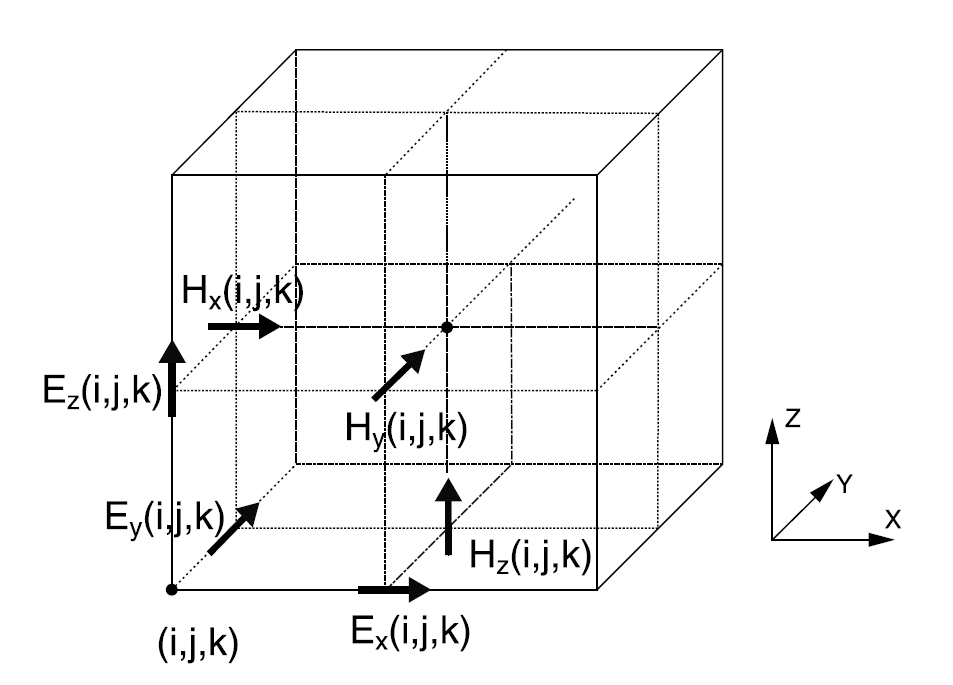
\includegraphics[width=1\textwidth]{include/graphics/image1}
\caption{Поля в ячейке сетки И}
\label{fig:YeeGrid}
\end{figure}

Так как существующие вычислительные мощности не позволяют организовать расчёт бесконечной сетки, на практике для численного решения какой-либо задачи электродинамики задают ограниченный счётный объём. \textit{Счётный объём} (или \textit{счётная область}) --- это та область пространства, в пределах которой выполняется численное моделирование, то есть осуществляется непосредственный расчёт электромагнитных полей.

Счётная область разбивается на ячейки при помощи сетки И; в каждом узле сетки задаются значения электрических и магнитных проницаемостей и проводимостей. Чаще всего в качестве базового материала счётного объёма рассматривают вакуум (или воздух), в отдельных узлах сетки помещаются металлические или диэлектрические структуры. Тем не менее, алгоритм вполне позволяет задать произвольные значения вышеперечисленных величин для каждой точки объёма.

Кроме того, для моделирования реальных задач необходимы источники поля: некоторая структура, способная создавать электромагнитное возмущение внутри счётного объёма. Так, среди прочего, метод конечных разностей во временной области позволяет симулировать возбуждение электромагнитных колебаний при помощи падающей электромагнитной волны либо точечного источника напряжения или тока.

Отличительной особенностью метода конечных разностей во временной области является его относительная простота. К достоинствам метода также можно отнести возможность создавать анимированные изображения распространения волновых процессов в счётном объеме, что может быть очень полезно для понимания происходящих в модели процессов и позволяет удостовериться в её корректности.

Основной недостаток метода --- обязательность разбиения счётного объёма на ячейки сетки И, причём величина шага дискретизации по пространственным координатам должна быть достаточно малой по сравнению с наименьшей длиной волны, встречающейся в конкретной задаче. Кроме того, эта величина ограничивает детализацию распределения материалов в пространстве, поэтому может оказаться, что счётный объём должен быть разделен на очень большое число ячеек, что влечёт за собой большие затраты памяти и увеличивает время моделирования.

Ещё одним недостатком метода конечных разностей во временной области является обязательность вычисления параметров поля в каждой точке счётного объёма. Так, при необходимости найти поле на некотором отдалении от источника придётся производить расчёт во всех точках, что находятся между источником и интересующей точкой.

К тому же, счётная область обязательно должна быть конечной. В большинстве случаев это достигается использованием искусственных граничных условий, но они, как правило, вызывают дополнительные искажения.

\subsection{Базовые уравнения}

Как уже было сказано, метод конечных разностей во временной области предполагает введение сетки, которая в простейшем случае представляет собой обыкновенный трёхмерный массив, в котором хранятся векторы полей и пространственная структура. Процедура расчёта заключается в поочерёдном обращении ко всем элементам этого массива в порядке возрастания индексов и последующем перевычислении его элементов с помощью базового алгоритма метода.

Для получения из дифференциальных уравнений Максвелла рассчитываемых численно выражений используется конечно-разностная схема, приведённая в 
работе~\cite{Schneider}.

Выражения для компонент магнитного поля:
\label{eq:BaseFdtdEquations}
\begin{align*}
	\Yee{H_x}{n+1/2}{i,j,k} &=
        \Yee{H_x}{n-1/2}{i,j,k} - \frac{\frac{\Delta{t}}{\mu}}
             {1+\frac{\sigma^{*}\Delta{t}}{2\mu}}
        \left[
            \frac{\yee{E_z}{n}{i,j+1,k} - \yee{E_z}{n}{i,j,k}}{\Delta{y}} -
            \frac{\yee{E_y}{n}{i,j,k+1} - \yee{E_y}{n}{i,j,k}}{\Delta{z}}
        \right], \\
	\Yee{H_y}{n+1/2}{i,j,k} &=
        \Yee{H_y}{n-1/2}{i,j,k} - \frac{\frac{\Delta{t}}{\mu}}
             {1+\frac{\sigma^{*}\Delta{t}}{2\mu}}
        \left[
            \frac{\yee{E_x}{n}{i,j,k+1} - \yee{E_x}{n}{i,j,k}}{\Delta{z}} -
            \frac{\yee{E_z}{n}{i+1,j,k} - \yee{E_z}{n}{i,j,k}}{\Delta{x}}
        \right], \\
	\Yee{H_z}{n+1/2}{i,j,k} &=
        \Yee{H_z}{n-1/2}{i,j,k} - \frac{\frac{\Delta{t}}{\mu}}
             {1+\frac{\sigma^{*}\Delta{t}}{2\mu}}
        \left[
            \frac{\yee{E_y}{n}{i+1,j,k} - \yee{E_y}{n}{i,j,k}}{\Delta{x}} -
            \frac{\yee{E_x}{n}{i,j+1,k} - \yee{E_x}{n}{i,j,k}}{\Delta{y}}
        \right].
\end{align*}

Выражения для компонент электрического поля:
\begin{align*}
	\fYee{E_x}{n+1}{i,j,k} &=
        \frac{1-\frac{\sigma\Delta{t}}{2\varepsilon}}
             {1+\frac{\sigma\Delta{t}}{2\varepsilon}} \fYee{E_x}{n}{i,j,k} +
        \frac{\frac{\Delta{t}}{\varepsilon}}
             {1+\frac{\sigma\Delta{t}}{2\varepsilon}}
        \left[
            \frac{\yee{H_z}{n+1/2}{i,j,k} - \yee{H_z}{n+1/2}{i,j-1,k}}{\Delta{y}} -
            \frac{\yee{H_y}{n+1/2}{i,j,k} - \yee{H_y}{n+1/2}{i,j,k-1}}{\Delta{z}}
        \right], \\
	\fYee{E_y}{n+1}{i,j,k} &=
        \frac{1-\frac{\sigma\Delta{t}}{2\varepsilon}}
	         {1+\frac{\sigma\Delta{t}}{2\varepsilon}} \fYee{E_y}{n}{i,j,k} +
        \frac{\frac{\Delta{t}}{\varepsilon}}
             {1+\frac{\sigma\Delta{t}}{2\varepsilon}}
        \left[
            \frac{\yee{H_x}{n+1/2}{i,j,k} - \yee{H_x}{n+1/2}{i,j,k-1}}{\Delta{z}} -
            \frac{\yee{H_z}{n+1/2}{i,j,k} - \yee{H_z}{n+1/2}{i-1,j,k}}{\Delta{x}}
        \right], \\
	\fYee{E_z}{n+1}{i,j,k} &=
        \frac{1-\frac{\sigma\Delta{t}}{2\varepsilon}}
             {1+\frac{\sigma\Delta{t}}{2\varepsilon}} \fYee{E_z}{n}{i,j,k} +
        \frac{\frac{\Delta{t}}{\varepsilon}}
             {1+\frac{\sigma\Delta{t}}{2\varepsilon}}
        \left[
            \frac{\yee{H_y}{n+1/2}{i,j,k} - \yee{H_y}{n+1/2}{i-1,j,k}}{\Delta{x}} -
            \frac{\yee{H_x}{n+1/2}{i,j,k} - \yee{H_x}{n+1/2}{i,j-1,k}}{\Delta{y}}
        \right].
\end{align*}

Выше приведены формулы, позволяющие вычислить каждую из компонент векторов напряжённости электрического и магнитного полей. В этих формулах используются следующие обозначения:
\begin{itemize}[label={}]
\item $ \sigma $ --- удельная электрическая проводимость материала в ячейке сетки;
\item $ \sigma^{*} $ --- удельная магнитная проводимость материала в ячейке сетки;
\item $ \varepsilon $ --- абсолютная диэлектрическая проницаемость материала;
\item $ \mu $ --- абсолютная магнитная проницаемость материала;
\item $ \Delta{t} $ --- шаг дискретизации по времени;
\item $ \Delta{x} $, $ \Delta{y} $, $ \Delta{z} $ --- шаги дискретизации по пространственным координатам.
\end{itemize}

Необходимо заметить, что величина $ \Delta{t} $ определяет частотные характеристики метода: наивысшая частота в спектре сигналов, распространение которых моделируется, не должна превышать $ f_{max} = \frac{1}{\Delta{t}} $.

Также величина $ \Delta{t} $ должна удовлетворять условию Куранта:
\begin{align*}
\Delta{t} < \frac{1}{c\sqrt{\frac{1}{\Delta{x}^2} + \frac{1}{\Delta{y}^2} + \frac{1}{\Delta{z}^2}}}
\end{align*}

Пересчёт значений компонент выполняется <<на месте>>, то есть рассчитанное в каждый последующий момент времени значение помещается в ту же ячейку сетки И, в которой находилось значение для предыдущего момента. Это позволяет несколько снизить требования к оперативной памяти, предъявляемые методом.

Однако приведённые выше базовые уравнения пригодны только для
бесконечной счётной области. Очевидно, произвести расчёт в такой области за конечное время невозможно, но существуют методы,
позволяющие получать решение электродинамической задачи при ограниченном счётном объёме. Среди них наибольшее распространение получили 
граничные условия идеального отражения и система \textit{идеально согласованных слоёв} (\textit{PML}).

Использование первого из этих методов приводит к многократному переотражению
сигнала внутри счётной области, два других позволяют существенно уменьшить 
отражение волны от границы. Граничные условия отражения намного проще, чем PML, однако система согласованных слоёв позволяет достичь на порядки меньшего
коэффициента отражения от границы счётного объёма.

\subsection{Условия идеального отражения}

Предположим, счётный объём окружён бесконечным идеальным проводником. Тогда 
напряжённости поля за пределами счётной области будут нулевыми, а 
электромагнитные волны, достигающие границ счётного объёма, будут полностью отражаться вовнутрь.

На практике это условие реализуется очень просто: счетный объём окружается
дополнительным слоем ячеек, поле в которых изначально
инициализируется нулями и никогда не высчитывается.

Однако данные граничные условия имеют серьёзный недостаток: чтобы отражённая от 
границ счётной области волна не вносила существенных искажений в происходящие внутри неё физические процессы, границы должны находиться достаточно далеко от интересующей нас области. Увеличение счётного объёма, в свою очередь, приводит к 
существенному увеличению времени расчёта и объёму оперативной памяти.

\subsection{Граничные условия PML}

Данный тип граничных условий (строго говоря, являющихся поглощающей приграничной областью, а не граничным условием, как таковым) считается 
одним из лучших на данный момент ввиду своей эффективности при использовании вкупе с неоднородными, дисперсионными, анизотропными и нелинейными 
средами~\cite{Taflove2005}. Основной идеей PML является окружение счётной области слоем анизотропного поглощающего материала, обладающего рядом особенностей.

Одной из таких особенностей является постоянство волнового сопротивления на границе раздела «счётная область --- согласованный слой» при равенстве $ \varepsilon $ 
и $ \mu $ по обе стороны границы и соблюдении следующего соотношения:
%%
\begin{align*}
\frac{\sigma}{\varepsilon} = \frac{\sigma^{*}}{\mu}.
\end{align*}

Электрическая и магнитная проводимость возрастают с увеличением расстояния
вглубь слоя PML по некоторому закону, называемому \emph{профилем потерь}.

В оригинальной работе Беренже~\cite{Berenger} был предложен следующий профиль потерь, как оптимальный по уровню отражения от границы раздела:
\begin{equation*}
%\label{eq:LossProfile}
\sigma_\text{PML}(i) = \left\{
\begin{array}{ll}
    \sigma_\text{PML}(0)\frac{\sqrt{g}-1}{\ln{g}}     & \text{при~} i=0,\\
    \sigma_\text{PML}(0)\frac{g-1}{\sqrt{g}\ln{g}}g^i & \text{при~} i=\frac12,1,\frac32,~\ldots
\end{array}
\right.
\end{equation*}
\begin{equation*}
\sigma_\text{PML}(0) = -\frac{\epsilon_0 \ln{g}} {2 d \epsilon_0\mu_0 (g^N-1)} \ln{r};\\
\end{equation*}
\begin{equation*}
\sigma^{*}_\text{PML}(i) = \frac{\mu}{\epsilon} \sigma_\text{PML}(i).
\end{equation*}

\noindent
В приведенных выше формулах использованы следующие обозначения:
\begin{itemize}[label={}]
\item $ \sigma_\text{PML}(i) $ --- электрическая проводимость $i$-го слоя;
\item $ \sigma^{*}_\text{PML}(i) $ --- магнитная проводимость $i$-го слоя;
\item $g$ --- подбираемый эмпирически параметр;
\item $r$ --- требуемый начальный коэффициент отражения;
\item $d$ --- интервал дискретизации пространства в данном направлении;
\item $N$ --- толщина слоя PML.
\end{itemize}

\noindent
Приблизительная оценка толщины слоя PML может быть получена из следующего
соотношения:
\begin{equation*}
%\label{eq:hz1}
    N= \frac{1}{\ln g} \ln
    \left[
        1 - \frac{\Theta t_p(\sqrt{g}-1)}{4\pi d \sqrt{\epsilon_0\mu_0}} \ln{r}
    \right],
\end{equation*}
где $t_p$ --- длительность процесса моделирования во времени,
а параметр~$\Theta$ подбираются эмпирически (обычно $\Theta\approx10$).

Ещё одной особенностью идеально согласованных слоёв является введения ограничения снизу на область допустимых частот. Сигналы с частотой, меньшей чем некоторое значение $f_{min}$, называемое \emph{частотой отсечки}, отражаются от границы PML. Ниже приведено выражение для частоты отсечки:
\begin{equation*}
%    \label{eq:PmlCutoffFrequency}
    f_{min} = \frac{\sigma_\text{PML}(0)}{2\pi\varepsilon_0}.
\end{equation*}

Основная идея получения базовых уравнений для расчета компонент поля
в согласованном слое состоит в том, что компоненты векторов $\vec{E}$
и $\vec{H}$ представляются в виде суммы двух слагаемых:
\begin{align*}
%\label{eq:PmlSplitFieldEquations}
    E_x = E_{xy}+E_{xz}, \\
    E_y = E_{yx}+E_{yz}, \\
    E_z = E_{zx}+E_{zy}, \\
    H_x = H_{xy}+H_{xz}, \\
    H_y = H_{yx}+H_{yz}, \\
    H_z = H_{zx}+H_{zy}.
\end{align*}
% TODO: Доверстать этот пиздец.
% \begin{пиздец}
\begin{eqnarray}
\label{eq:pml13}
%---
\left\{
\begin{array}{rcl}
  %--- xy
  \varepsilon \frac{\partial}{\partial t}E_{xy} + \sigma_y E_{xy} & = & \frac{\partial}{\partial y}(H_{zx}+H_{zy}) \\
  %--- xz
  \varepsilon \frac{\partial}{\partial t}E_{xz} + \sigma_z E_{xz} & = & \frac{\partial}{\partial z}(H_{yz}+H_{yx}) \\
  %--- yz
  \varepsilon \frac{\partial}{\partial t}E_{yz} + \sigma_z E_{yz} & = & \frac{\partial}{\partial z}(H_{xy}+H_{xz}) \\
  %--- yx
  \varepsilon \frac{\partial}{\partial t}E_{yx} + \sigma_x E_{yx} & = & \frac{\partial}{\partial x}(H_{zx}+H_{zy}) \\
  %--- zx
  \varepsilon \frac{\partial}{\partial t}E_{zx} + \sigma_x E_{zx} & = & \frac{\partial}{\partial x}(H_{yx}+H_{yz}) \\
  %--- zy
  \varepsilon \frac{\partial}{\partial t}E_{zy} + \sigma_y E_{zy} & = & \frac{\partial}{\partial y}(H_{xy}+H_{xz}) \\
\end{array}
\right.
\end{eqnarray}
\begin{eqnarray}
\label{eq:pml14}
\left\{
\begin{array}{rcl}
  %--- xy
  \varepsilon \frac{\partial}{\partial t}H_{xy} + \sigma_y^* H_{xy} & = & \frac{\partial}{\partial y}(E_{zx}+E_{zy}) \\
  %--- xz
  \varepsilon \frac{\partial}{\partial t}H_{xz} + \sigma_z^* H_{xz} & = & \frac{\partial}{\partial z}(E_{yz}+E_{yx}) \\
  %--- yz
  \varepsilon \frac{\partial}{\partial t}H_{yz} + \sigma_z^* H_{yz} & = & \frac{\partial}{\partial z}(E_{xy}+E_{xz}) \\
  %--- yx
  \varepsilon \frac{\partial}{\partial t}H_{yx} + \sigma_x^* H_{yx} & = & \frac{\partial}{\partial x}(E_{zx}+E_{zy}) \\
  %--- zx
  \varepsilon \frac{\partial}{\partial t}H_{zx} + \sigma_x^* H_{zx} & = & \frac{\partial}{\partial x}(E_{yx}+E_{yz}) \\
  %--- zy
  \varepsilon \frac{\partial}{\partial t}H_{zy} + \sigma_y^* H_{zy} & = & \frac{\partial}{\partial y}(E_{xy}+E_{xz}) \\
\end{array}
\right.
\end{eqnarray}

Анизотропия согласованного слоя проявляется в следующем: каждой ячейке соответствует набор $(\sigma_x,\sigma_y,\sigma_z)$, причем элемент $\sigma_\alpha$ ($\alpha={x,y,z}$) не равен нулю только для ячеек слоя, пересекаемого соответствующей осью координат~(рис.~\ref{fig:PML}).

% Рисунок 2 -- Анизотропия PML
\afterpage{\clearpage}
\begin{figure}[p]
\centering
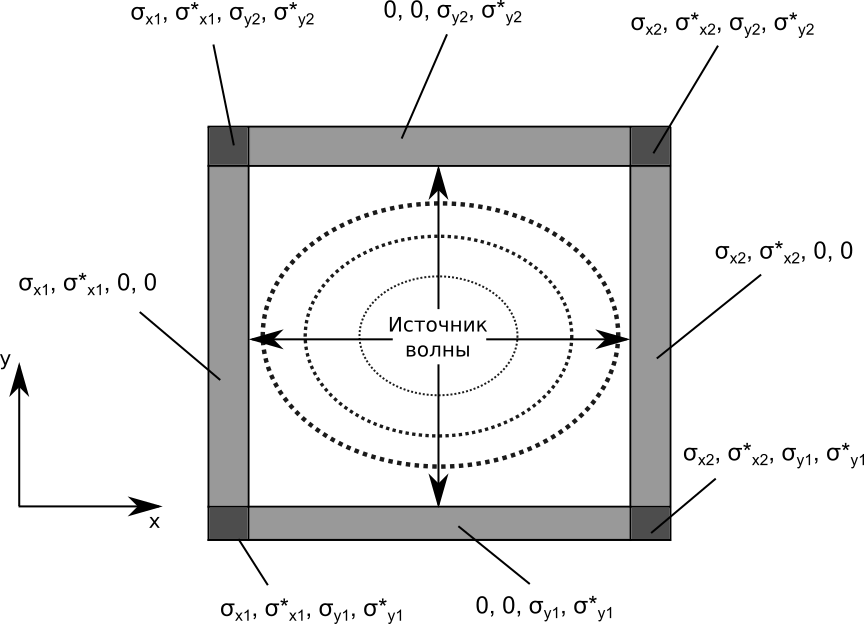
\includegraphics[width=1\textwidth]{include/graphics/image4195}
\caption{Анизотропия PML}
\label{fig:PML}
\end{figure}

В дискретной форме системы уравнений (\ref{eq:pml13}) и (\ref{eq:pml14}) выглядят следующим образом:
\begin{equation*}
\left\{
\begin{aligned}
H_{xy (i,j,k)}^{n+1} = D_{ay (i,j,k)} H_{xy (i,j,k)}^{n} - D_{by (i,j,k)}
\left[
    \frac{E_{z (i,j+1,k)}^n - E_{z (i,j,k)}^n}{\Delta y}
\right], \\
%---
H_{xz (i,j,k)}^{n+1} = D_{az (i,j,k)} H_{xz (i,j,k)}^{n} - D_{bz (i,j,k)}
\left[
    \frac{E_{y (i,j,k+1)}^n - E_{y (i,j,k)}^n}{\Delta z}
\right], \\
%---
H_{yx (i,j,k)}^{n+1} = D_{ax (i,j,k)} H_{yx (i,j,k)}^{n} - D_{bx (i,j,k)}
\left[
    \frac{E_{z (i+1,j,k)}^n - E_{z (i,j,k)}^n}{\Delta x}
\right], \\
%---
H_{yz (i,j,k)}^{n+1} = D_{az (i,j,k)} H_{yz (i,j,k)}^{n} - D_{bz (i,j,k)}
\left[
    \frac{E_{x (i,j,k+1)}^n - E_{x (i,j,k)}^n}{\Delta z}
\right], \\
%---
H_{zx (i,j,k)}^{n+1} = D_{ax (i,j,k)} H_{zx (i,j,k)}^{n} - D_{bx (i,j,k)}
\left[
    \frac{E_{y (i+1,j,k)}^n - E_{z (i,j,k)}^n}{\Delta x}
\right], \\
%---
H_{zy (i,j,k)}^{n+1} = D_{ay (i,j,k)} H_{zy (i,j,k)}^{n} - D_{by (i,j,k)}
\left[
    \frac{E_{x (i,j+1,k)}^n - E_{x (i,j,k)}^n}{\Delta y}
\right].
\end{aligned}
\right.
\end{equation*}

\begin{equation*}
\left\{
\begin{aligned}
E_{xy (i,j,k)}^{n+1} = C_{ay (i,j,k)} E_{xy (i,j,k)}^{n} - C_{by (i,j,k)}
\left[
    \frac{H_{z (i,j,k)}^{n+1} - H_{z (i,j-1,k)}^{n+1}}{\Delta y}
\right], \\
%---
E_{xz (i,j,k)}^{n+1} = C_{az (i,j,k)} E_{xz (i,j,k)}^{n} - C_{bz (i,j,k)}
\left[
    \frac{H_{y (i,j,k)}^{n+1} - H_{y (i,j,k-1)}^{n+1}}{\Delta z}
\right], \\
%---
E_{yx (i,j,k)}^{n+1} = C_{ax (i,j,k)} E_{yx (i,j,k)}^{n} - C_{bx (i,j,k)}
\left[
    \frac{H_{z (i,j,k)}^{n+1} - H_{z (i-1,j,k)}^{n+1}}{\Delta x}
\right], \\
%---
E_{yz (i,j,k)}^{n+1} = C_{az (i,j,k)} E_{yz (i,j,k)}^{n} - C_{bz (i,j,k)}
\left[
    \frac{H_{x (i,j,k)}^{n+1} - H_{x (i,j,k-1)}^{n+1}}{\Delta z}
\right], \\
%---
E_{zx (i,j,k)}^{n+1} = C_{ax (i,j,k)} E_{zx (i,j,k)}^{n} - C_{bx (i,j,k)}
\left[
    \frac{H_{y (i,j,k)}^{n+1} - H_{z (i-1,j,k)}^{n+1}}{\Delta x}
\right], \\
%---
E_{zy (i,j,k)}^{n+1} = C_{ay (i,j,k)} E_{zy (i,j,k)}^{n} - C_{by (i,j,k)}
\left[
    \frac{H_{x (i,j,k)}^{n+1} - H_{x (i,j-1,k)}^{n+1}}{\Delta y}
\right].
\end{aligned}
\right.
\end{equation*}

Коэффициенты~$C$ и~$D$ уравнениях выше вычисляются по формулам:
\begin{equation*}
\begin{aligned}
D_{ax (i,j,k)} =
\frac
{
    1-\frac{\sigma_{x (i,j,k)}^*\Delta t}{2\mu_{(i,j,k)}}
}{
    1+\frac{\sigma_{x (i,j,k)}^*\Delta t}{2\mu_{(i,j,k)}}
}, \\
%---
D_{bx (i,j,k)} =
\frac
{
    \frac{\Delta t}{\mu_{(i,j,k)}}
}{
    1+\frac{\sigma_{x (i,j,k)}^*\Delta t}{2\mu_{(i,j,k)}}
},
\end{aligned}
%---------------
\quad
\begin{aligned}
D_{ay (i,j,k)} =
\frac
{
    1-\frac{\sigma_{y (i,j,k)}^*\Delta t}{2\mu_{(i,j,k)}}
}{
    1+\frac{\sigma_{y (i,j,k)}^*\Delta t}{2\mu_{(i,j,k)}}
}, \\
%---
D_{by (i,j,k)} =
\frac
{
    \frac{\Delta t}{\mu_{(i,j,k)}}
}{
    1+\frac{\sigma_{y (i,j,k)}^*\Delta t}{2\mu_{(i,j,k)}}
},
\end{aligned}
%---------------
\quad
\begin{aligned}
D_{az (i,j,k)} =
\frac
{
    1-\frac{\sigma_{z (i,j,k)}^*\Delta t}{2\mu_{(i,j,k)}}
}{
    1+\frac{\sigma_{z (i,j,k)}^*\Delta t}{2\mu_{(i,j,k)}}
}, \\
%---
D_{bz (i,j,k)} =
\frac
{
    \frac{\Delta t}{\mu_{(i,j,k)}}
}{
    1+\frac{\sigma_{z (i,j,k)}^*\Delta t}{2\mu_{(i,j,k)}}
},
\end{aligned}
%---------------
\end{equation*}

\begin{equation*}
\begin{aligned}
C_{ax (i,j,k)} =
\frac
{
    1-\frac{\sigma_{x (i,j,k)}\Delta t}{2\varepsilon_{(i,j,k)}}
}{
    1+\frac{\sigma_{x (i,j,k)}\Delta t}{2\varepsilon_{(i,j,k)}}
}, \\
%---
C_{bx (i,j,k)} =
\frac
{
    \frac{\Delta t}{\varepsilon_{(i,j,k)}}
}{
    1+\frac{\sigma_{x (i,j,k)}\Delta t}{2\varepsilon_{(i,j,k)}}
},
\end{aligned}
%---------------
\quad
\begin{aligned}
C_{ay (i,j,k)} =
\frac
{
    1-\frac{\sigma_{y (i,j,k)}\Delta t}{2\varepsilon_{(i,j,k)}}
}{
    1+\frac{\sigma_{y (i,j,k)}\Delta t}{2\varepsilon_{(i,j,k)}}
}, \\
%---
C_{by (i,j,k)} =
\frac
{
    \frac{\Delta t}{\varepsilon_{(i,j,k)}}
}{
    1+\frac{\sigma_{y (i,j,k)}\Delta t}{2\varepsilon_{(i,j,k)}}
},
\end{aligned}
%---------------
\quad
\begin{aligned}
C_{az (i,j,k)} =
\frac
{
    1-\frac{\sigma_{z (i,j,k)}\Delta t}{2\varepsilon_{(i,j,k)}}
}{
    1+\frac{\sigma_{z (i,j,k)}\Delta t}{2\varepsilon_{(i,j,k)}}
}, \\
%---
C_{bz (i,j,k)} =
\frac
{
    \frac{\Delta t}{\varepsilon_{(i,j,k)}}
}{
    1+\frac{\sigma_{z (i,j,k)}\Delta t}{2\varepsilon_{(i,j,k)}}
},
\end{aligned}
%---------------
\end{equation*}

% \end{пиздец}

Следует заметить, что в реальной ситуации всегда присутствуют
отражения.
Они складываются из:
\begin{itemize}
  \item отражений от первого слоя PML;
  \item отражений между слоями PML;
  \item отражений от проводящей границы за последним слоем PML.
\end{itemize}

\noindent
В связи с этим, для уменьшения отражения от первого слоя добиваются малого значения~$\sigma_0$. Отражения между слоями подавляются за счет
ограничения скорости роста профиля потерь. Для уменьшения влияния волны,
отраженной от бесконечно проводящей границы, увеличивают число слоёв PML.

\subsection{Точечный резистивный источник напряжения}

Возможность моделировать сосредоточенные элементы вводится дополнительно, при этом границы применения метода существенно расширяются. В частности, точечный генератор напряжения с заданным внутренним сопротивлением оказывается весьма удобной моделью источника питания.

Достоинством этого дополнения метода конечных разностей во временной области является то, что вид уравнений меняется весьма незначительно. Если источник ориентирован вдоль оси $Z$, то в системе уравнений Максвелла~\eqref{eq:MaxwellEquations} изменится только одна составляющая векторного уравнения для ротора вектора магнитной напряжённости:

\begin{equation}
    \label{eq:LumpedSource:MaxwellEquationsAmendment}
    (\Rot\vec{H})_z = \varepsilon\frac{\partial{E_z}}{\partial{t}} +
        \sigma E_z + \frac{I_L}{\Delta{x}\Delta{y}},
\end{equation}
где $ I_L $ --- ток через источник.

Подвергнув уравнение~\eqref{eq:LumpedSource:MaxwellEquationsAmendment} действию конечно-разностной схемы и положив~$\sigma_E=0$, получим следующую формулу:
\begin{multline}
    \label{eq:LumpedSource:FdtdEquationsAmendmentWithI}
    \fYee{E_z}{n+1}{i,j,k} = \fYee{E_z}{n}{i,j,k} +
        \frac{\Delta{t}}{\yee{\varepsilon}{}{i,j,k}}
        \left[
            \frac{\yee{H_y}{n+1}{i,j,k}-\yee{H_y}{n+1}{i-1,j,k}}{\Delta{x}} -
            \frac{\yee{H_x}{n+1}{i,j,k}-\yee{H_x}{n+1}{i,j-1,k}}{\Delta{y}}
        \right] - \\ -
        \frac{\yee{I_L}{n+1}{}\Delta{t}}
             {\yee{\varepsilon}{}{i,j,k}\Delta{x}\Delta{y}}.
\end{multline}

Формула~\ref{eq:LumpedSource:FdtdEquationsAmendmentWithI} позволяет моделировать точечный источник тока внутри счётного объёма.

Согласно закону Ома и работе~\cite{Makinen}, для рассматриваемого сосредоточенного генератора напряжения
с внутренним сопротивлением $R$ будет иметь место равенство
\begin{equation}
    \label{eq:LumpedSource:OhmLaw}
    \fYee{I_L}{n+1}{} = \frac{\Delta{z}}{2R}
    \left(
        \fYee{E_z}{n+1}{i,j,k} - \Yee{E_z}{n}{i,j,k}
    \right) +
    \frac{\yee{U_s}{n+1}{}}{R},
\end{equation}
где $U_s$ --- генерируемое источником напряжение.

После подстановки~\eqref{eq:LumpedSource:OhmLaw}
в~\eqref{eq:LumpedSource:FdtdEquationsAmendmentWithI} получим простое уравнение
для~$E_z$:
\begin{multline*}
    \label{eq:LumpedSource:FdtdEquationsAmendmentWithU}
    \fYee{E_z}{n+1}{i,j,k} =
        \fYee{C_E}{}{i,j,k}\fYee{E_z}{n}{i,j,k}~~+~~
        \Yee{C_H}{}{i,j,k}
        \left[
            \frac{\yee{H_y}{n+1}{i,j,k}-\yee{H_y}{n+1}{i-1,j,k}}{\Delta{x}}
        \right. - \\ -
        \left.
            \frac{\yee{H_x}{n+1}{i,j,k}-\yee{H_x}{n+1}{i,j-1,k}}{\Delta{y}} -
            \frac{\yee{U_s}{n+1}{}}{R\Delta{x}\Delta{y}}
        \right],
\end{multline*}
где $C_E$ и~$C_H$ определяются по следующим формулам:
\begin{equation*}
    \newcommand\XA{\displaystyle
        \frac{\Delta{t}}{\yee{\varepsilon}{}{i,j,k}}}
    \newcommand\XB{\displaystyle
        \frac{\Delta{t}\Delta{z}}{2R\yee{\varepsilon}{}{i,j,k}\Delta{x}\Delta{y}}}
    % --
    \fYee{C_E}{}{i,j,k} = \frac{1-\XB}{1+\XB}, \quad
    \fYee{C_H}{}{i,j,k} = \frac{\XA}{1+\XB}.
\end{equation*}

Формулы для прочих компонент остаются неизменными.
\clearpage